\subsubsection{ipconfig}
\begin{figure}[H]
  \begin{center}
      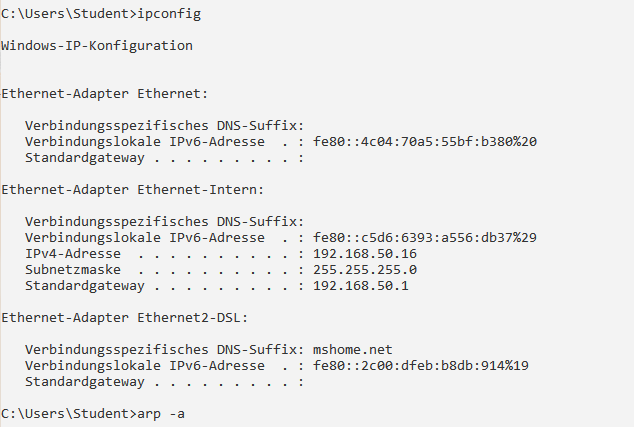
\includegraphics[width=0.618\textwidth]{graphics/versuch/3_2/ipconfig}
      \caption{Ausgabe des CMD-Befehls \textit{ipconfig}}\label{abb_2}
  \end{center}
\end{figure}

Der Befehl \inlinecode{ipconfig} zeigt die IP-Konfigurationen der Netzwerkschnittstellen unter Windows an. Für die folgenden Betrachtungen ist das Interface \glqq Ethernet-Adapter Ethernet-Intern\grqq\ relevant. Aus Abbildung \ref{abb_2} kann man dessen zugewiesene IP-Adresse \inlinecode{192.168.20.16}, welche das Interface im Netzwerk für IP-Pakete identifiziert. Ob diese statisch oder dynamisch (DHCP) zugewiesen wurde, ist hieraus nicht erkennbar. \\

Außerdem angezeigt ist die Subnetzmaske \inlinecode{255.255.255.0}. Diese trennt den IP-Adressbereich in Netzwerk- und Hostbereich auf, um im gleichen physischen Netzwerk mehrere Unternetze (Subnets) zu erzeugen. Ziel-IP-Adresse und Subnetzmaske werden logisch UND-verknüpft, wodurch man die Netzadresse des Ziels erhält. Ist das Ergebnis gleich der eigenen Netzadresse, kann das Paket direkt an den entsprechenden Host versandt werden. Stimmt es nicht überein, wird es an den \emph{Default Gateway} gesandt, welcher das Paket weiterleitet.\\

Die Netzadresse der Schnittstelle aus Abb. \ref{abb_2} ist also \inlinecode{192.168.50.0/24} (x.x.x.0 immer reserviert als Netzadresse), die Adresse des Standardgateways ist \inlinecode{192.168.50.1}.

\subsubsection{arp -a}\label{A3.2.2}
\begin{figure}[H]
  \begin{center}
      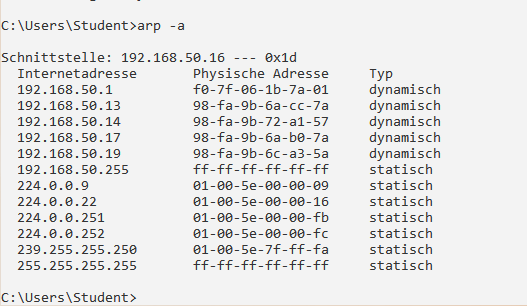
\includegraphics[width=0.618\textwidth]{graphics/versuch/3_2/arp_a}
      \caption{Ausgabe des CMD-Befehls arp -a}\label{abb_arp}
  \end{center}
\end{figure}

Mit dem Befehl \inlinecode{arp -a} (ARP: Address Resolution Protocol) kann unter Windows die Routingtabelle (Cache) angezeigt werden. Diese enthält die Zuweisungen der IP-Adressen zu den MAC- bzw. physischen Adressen, sowie, ob diese dynamisch oder statisch eingerichtet wurden. Diese Tabelle wird von Schicht 2 genutzt, um Ziel-IP-Adressen (Schicht 3) in (lokale) Hardwareadressen zu übersetzen.\\

In Abbildung \ref{abb_arp} erkennt man die Einträge der im gleichen Netz (\inlinecode{192.168.50.0}) befindlichen Geräte. Dazu zählen sowohl weitere Hosts, wie z.B. \inlinecode{192.168.50.17}, als auch der Default Gateway und die Broadcast-Adresse \inlinecode{192.168.50.255}/\inlinecode{ff-ff-ff-ff-ff-ff}, welche u.a. für ARP-Anfragen verwendet wird, um eine IP-Adresse in eine physische Adresse umzuwandeln, sollte sie nicht in der Tabelle aufgeführt sein. Die Broadcast-Adresse für einen Host lässt sich berechnen: Zuerst wird die Subnetzmaske negiert und dann ODER-verknüpft mit der Host-Adresse.

\begin{figure}[H]
\centering
\resizebox{\textwidth}{!}{\import{graphics/}{v_broadcast_calc.pdf_tex}}
\end{figure}

Das Ergebnis deckt sich mit der Adresse aus Abbildung \ref{abb_arp}.\\

Auffällig sind weiterhin die folgenden \inlinecode{224.0.0.x}-Adressen, sowie die Adresse \inlinecode{239.255.255.250}. Diese sind Multicast-Adressen (siehe \ref{A4.9}). IPv4 reserviert einen Multicast-Adressbereich von \inlinecode{224.0.0.0} bis \inlinecode{239.255.255.255}, in welchen diese Adressen gerade fallen.\\

Da der letzte Eintrag ebenfalls auf die physische Adresse \inlinecode{ff-ff-ff-ff-ff-ff} abgebildet ist, ist klar, dass es sich hierbei ebenfalls um eine Broadcast-Adresse handeln muss, sie ist ebenfalls reserviert.
